\documentclass[a4paper]{article}
\usepackage{amsmath, amssymb, amsfonts}
\usepackage[margin=1in]{geometry}
\usepackage{graphicx}
\usepackage{tikz}
\usepackage{esint}
\setlength{\parindent}{0em}
\setlength{\parskip}{1ex}
\newcommand{\vct}[1]{\overrightarrow{#1}}
\newcommand{\dif}{\,\mathrm{d}}
\newcommand{\pd}[2]{\frac{\partial {#1}}{\partial {#2}}}
\newcommand{\dd}[2]{\frac{\mathrm{d} {#1}}{\mathrm{d} {#2}}}
\newcommand{\C}{\mathbb{C}}
\newcommand{\R}{\mathbb{R}}
\newcommand{\Q}{\mathbb{Q}}
\newcommand{\Z}{\mathbb{Z}}
\newcommand{\N}{\mathbb{N}}
\newcommand{\fn}[3]{{#1}\colon {#2} \rightarrow {#3}}
\newcommand{\avg}[1]{\langle {#1} \rangle}
\newcommand{\Sum}[2][0]{\sum_{{#2} = {#1}}^{\infty}}
\newcommand{\Lim}[1]{\lim_{{#1} \rightarrow \infty}}
\newcommand{\Binom}[2]{\begin{pmatrix} {#1} \cr {#2} \end{pmatrix}}
\newcommand{\duline}[1]{\underline{\underline{#1}}}

\begin{document}
\paragraph{Naloga.} Gibanje delca ob širjenju zvoka. Tekočina, po kateri se zvok širi, ima hitrost
$v_t = v_0 \cos\omega t$. Na delec deluje tudi sila upora $F_u = 6\pi R \eta (v_z - v)$. Iščemo $v(t)$.
$$m\dot v = 6\pi R \eta (v_0\cos(\omega t) - v)$$
$$m \dot v + 6 \pi R \eta v = 6\pi R \eta v_0\cos\omega t$$
Označimo $1/\tau = 6\pi R \eta / m$.
$$\dot v + \frac{v}{\tau} = \frac{v_0}{\tau}\cos\omega t$$
Homogena rešitev:
$$v = Ae^{-t/\tau}$$
Partikularna rešitev: Vzamemo nastavek $v = Be^{i \omega t}$
$$i\omega Be^{i\omega t} + Be^{i\omega t}\frac{1}{\tau} = \frac{v_0}{\tau}\,\mathfrak{Re}\left[e^{i\omega t}\right]$$
$$B = \frac{v_0}{\tau}\left[iw + \frac{1}{\tau}\right]^{-1}$$
$$v(t) = Ae^{-t/\tau} + \frac{v_0}{\tau}\,\mathfrak{Re}\left[\frac{1}{1/\tau + i\omega}e^{i\omega t}\right]$$
Po potrebi vstavimo robne pogoje. Izraz v oklepaju lahko še malo polepšamo in dobimo končno rešitev
$$v(t) = \frac{v_0}{\tau}\left[\frac{1}{\tau\left(1/\tau^2 + \omega^2\right)}\cos\omega t +
\frac{\omega}{1/\tau^2 + \omega^2}\sin\omega t\right] + Ae^{-t/\tau}$$
\paragraph{Naloga.} Telo je povezano z vzmetmi, kot kaže skica:
\begin{figure}[h!]
    \centering
    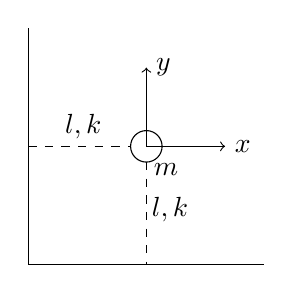
\begin{tikzpicture}
        \draw (0, 3) -- (0, 0) -- (3, 0);
        \draw[dashed] (0, 1.5) -- (1.3, 1.5);
        \draw (1.5, 1.5) circle (0.2);
        \draw[dashed] (1.5, 1.3) -- (1.5, 0);
        \draw[->] (1.5, 1.5) -- (2.5, 1.5) node[right] {$x$};
        \draw[->] (1.5, 1.5) -- (1.5, 2.5) node[right] {$y$};
        \node (m) at (1.75, 1.2) {$m$};
        \node (lk) at (1.8, 0.7) {$l,k$};
        \node (lk) at (0.7, 1.75) {$l,k$};
    \end{tikzpicture}
\end{figure}
\newline
Iščemo lastna nihanja pri majhnih odmikih. Privzamemo, da gravitacija na sistem nima vpliva.
$$F = k(l-l') = k\left(\sqrt{l^2 + x^2} - l\right) \approx k\left[l + \frac{1}{2l}x - l\right] = \frac{kx^2}{2l}$$
$$F_x = -F\cos\alpha = -F\frac{x}{\sqrt{l^2 + x^2}}$$
$$F_y = -F\sin\alpha = -F\frac{l}{\sqrt{l^2 + x^2}}$$
Te sile so reda velikosti $\mathcal{O(x^2/l^2)}$. Pri dovolj majhnih $x$ so ti popravki zanemarljivi in lahko uporabimo kar
$$m\ddot{x} = -kx$$
$$m\ddot{y} = -ky$$
Sistem ima rešitev $\vct{X} = \vct{X_0}e^{i\omega t}$
\end{document}